
\subsection{スマホアプリによる仮想ビーコンとビーコンデバイスの併用}

 BLEビーコンの利用には複数のメリットとデメリットが存在する,スマホアプリによる仮想ビーコンとビーコンデバイスの併用によってメリットを維持した状態でデメリットを解消する.
 ビーコンデバイスを導入するメリットとしてユーザの意識的な記録動作を要しない点が挙げられる.
一方デメリットとしてビーコンデバイスの電池切れによって動作が停止する点,ビーコンデバイスの設定及び状態の把握に専用のアプリケーションによる接続を要する点,まず,ビーコンデバイスは電池切れによって動作が停止してしまう.
在室情報を継続的に記録するために,BLEビーコンは常時動作する必要がある.
そのためビーコンデバイスの電池切れになった場合はユーザにslackによる通知などで電池交換を促していた.
しかし電池交換はユーザに委ねられているため,電池交換の手間からに電池切れを起こしたままのビーコンデバイスが放置される状況が存在した.
結果,システムの可用性が損なわれていた.

 ビーコンデバイスの電池を把握する場合,ビーコンデバイス一台づつに専用のアプリを用いた接続を行い電池残量を確認する必要があった.
またメーカーはビーコンデバイスに接続するライブラリの公開に否定的であり,電池残量の把握を容易には行えない.
我々はビーコンデバイスを導入するメリットを維持した状態でデメリットを解決させる方法としてスマホアプリによる仮想ビーコンとビーコンデバイスの併用とそれに伴うAndroid向けのアプリケーションを作成した.
 現代においてスマートフォンは所持するインフラであり,本研究の対象とするユーザ層は可能な限りスマートフォンの電池状態に配慮する性質を持つ.
また,電池切れを外見上で判断不能なビーコンとは異なり画面表示などによって電池残量が判断可能である.
その性質を踏まえビーコンデバイスのメリットであるユーザの意識的な記録動作を要しない点を維持するためにアプリケーションのバックグラウンド動作を行った.
 既存の研究では入退室を記録時に自身でアプリケーションを起動し記録する方式が採用されているが,我々の行っているビーコンデバイスを携帯する方式の場合ユーザの記録動作なしで行われるためユーザの協力を得やすく,またヒューマンエラーを防止できる.
その利点を維持するために,アプリケーションを起動しビーコンの動作を開始した後は図2に示す通りスマートフォンの通知領域に動作状況を表示し,ユーザのそれ以上の操作を要しない.
通知領域への表示はビーコンとしての動作と連携しており, アプリケーションの動作中は永続的に表示される.
よってアプリケーションが停止した場合もユーザによる判別が容易であるため,ユーザによる動作の再開が容易である.
これによって電池切れによる動作が停止する問題とビーコンデバイスが専用アプリケーションを要求する問題を解消している.

\begin{figure}[tbh]
  \centering
  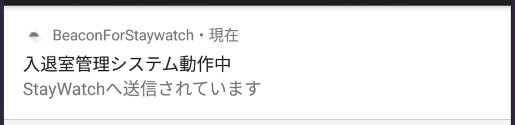
\includegraphics[width=8cm]{image/notify.jpg}
  \caption{通知領域による可視化}
  \label{multipleBPM}
\end{figure}
 しかしスマホアプリによる仮想ビーコンのみを利用する場合,様々な状況のユーザの継続した利用が困難であるため,ビーコンデバイスと併用できる仕様とした.
 普段から継続的に利用する滞在ウォッチユーザにとっては,ビーコンデバイスは先述の通り電池交換の手間がある.
スマホアプリはそのようなユーザにとっては,電池交換の手間がないため有用である.
 しかしスマホアプリのインストールに抵抗があるユーザやインストールができないユーザも想定される.
例としてはスマートフォンを持っていないユーザ,アプリの使用に伴うバッテリーの消費気が気になるユーザなどが上げられる.

 これらの問題はビーコンデバイスとスマホアプリによる仮想ビーコンをハイブリット化することで解決できる.
スマホアプリ内で利用するUUIDをビーコンデバイスで使用するUUIDと同じ値に設定し同じユーザの在室情報を記録している.
この方法はスマートフォンかビーコンデバイスのどちらかを持っていればよいため継続的にデータを記録する観点から見ても有用である.













